\documentclass[12pt]{beamer}
\usepackage[utf8]{inputenc}
\usepackage[spanish]{babel}
\usepackage{amsmath}
\usepackage{amsfonts}
\usepackage{amssymb}
\usepackage{graphicx}
\usepackage{mathrsfs} 
\usepackage{outlines}
\usetheme{Goettingen}
%\usepackage{subfig,graphicx,showframe}
\setbeamertemplate{bibliography item}[text]
\DeclareMathOperator{\re}{Re}
\begin{document}
	\author{Carlos Daniel Contreras Quiroz}
	\title{Desarrollo de un programa de lectura y análisis de películas radiocrómicas para verificación dosimétrica}
	%\subtitle{}
	\logo{
\includegraphics{images/logo.png}}
	\institute{Universidad de los Andes}
	%\date{}
	%\subject{}
	%\setbeamercovered{transparent}
	%\setbeamertemplate{navigation symbols}{}
	\begin{frame}[plain]
	\maketitle
\end{frame}

\begin{frame}{Contenido}
\tableofcontents
\end{frame}

\section{Introducción}
\begin{frame}
\vfill
\centering
\begin{beamercolorbox}[sep=8pt,center,shadow=true,rounded=true]{title}
	\usebeamerfont{title}\insertsectionhead\par%
\end{beamercolorbox}
\vfill
\end{frame}
\subsection{Objetivos}

\begin{frame}{Motivación}
Los planes de tratamiento con radioterapia requieren de una alta precisión en las dosis entregadas, desviaciones menores al $5\%$.  \\~\\

\begin{figure}
	\centering
	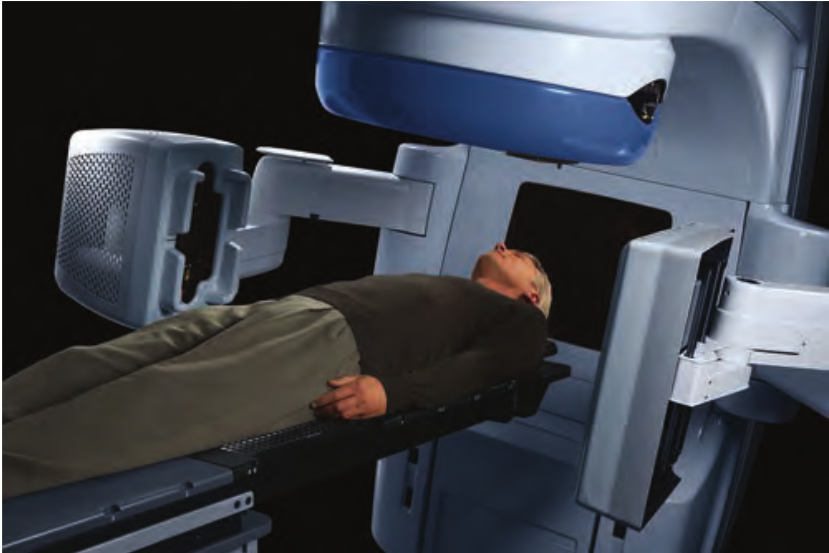
\includegraphics[width=0.7\linewidth]{images/paciente.png}
	\caption{Maquina Varian Trylogy \cite{khan2014the}}
\end{figure}

\end{frame}

\begin{frame}{Motivación}
	Existen diversos mecanismos para realizar el monitoreo de distribuciones y dosis entregadas.\\
\end{frame}

\begin{frame}{Motivación}
	Cámaras de ionización 
	\begin{figure}
		\centering
		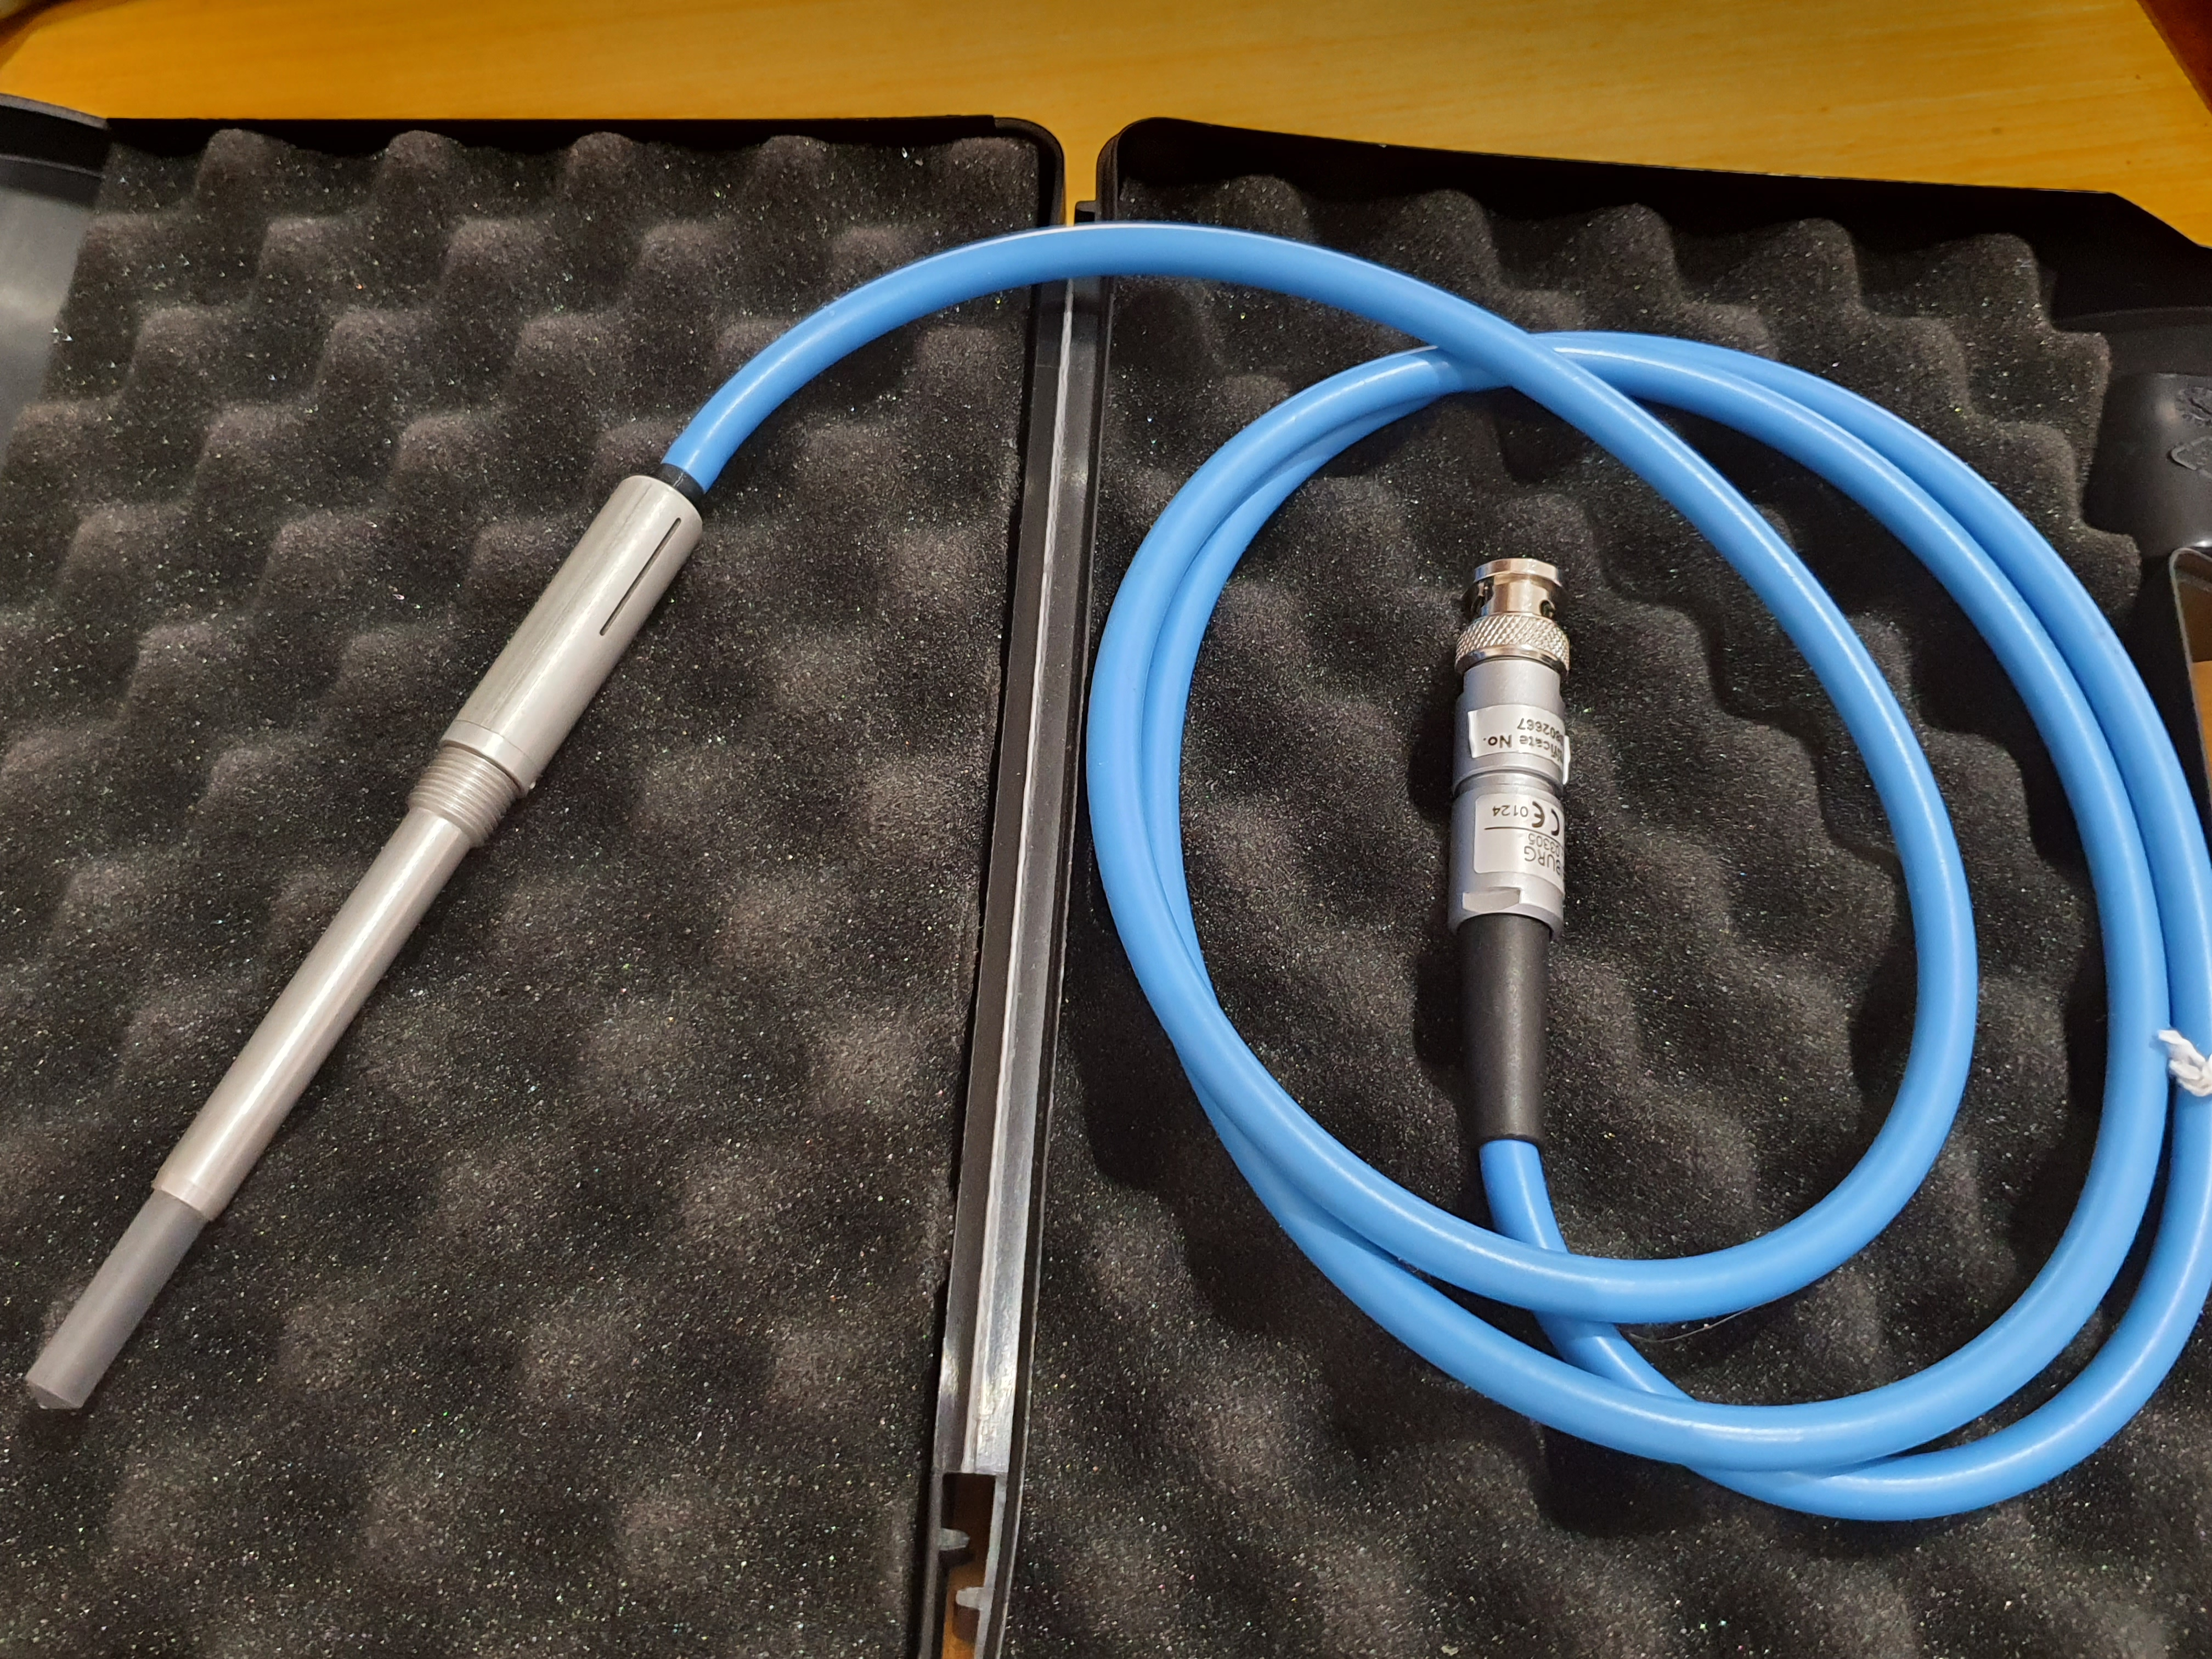
\includegraphics[width=0.7\linewidth]{images/camara.jpg}
	\end{figure}
\end{frame}

\begin{frame}{Motivación}
Paneles de silicio
\begin{figure}
	\centering
	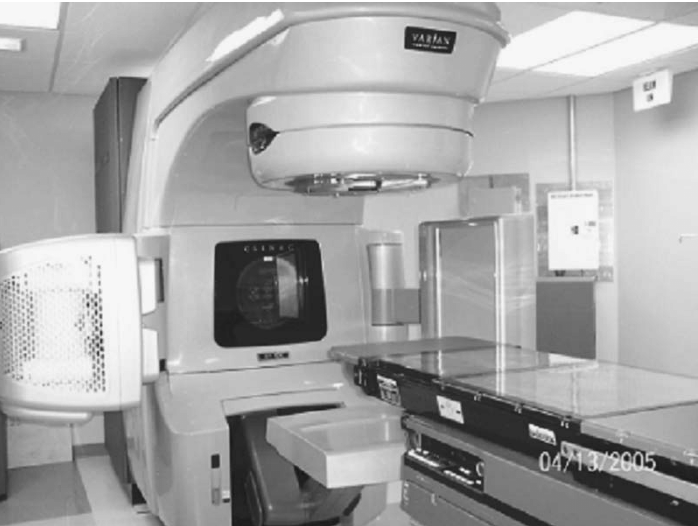
\includegraphics[width=0.7\linewidth]{images/silicio.png}
	\caption{\cite{Yoo2006}}
\end{figure}
\end{frame}

\begin{frame}
	Sin embargo, no sirven en todos los casos
	\begin{itemize}
		\item No tiene la resolución espacial suficiente para procedimientos como radiocirugia
		\item Son demasiado costos y poco asequibles 
	\end{itemize}
\end{frame}

\begin{frame}{Motivación}
	Una posible solución es el uso de películas radiocrómicas
\begin{figure}[htp]% [H] is so declass\'e!
	\centering
	\begin{minipage}{0.45\textwidth}
		
\includegraphics[width=\textwidth]{images/fondoblancoLandscape-1.png}
		\caption{Película EBT2}
	\end{minipage}\hfill
	\begin{minipage}{0.45\textwidth}
		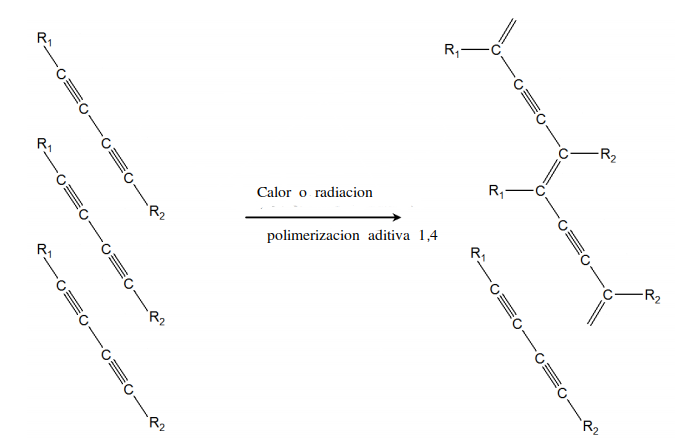
\includegraphics[width=\textwidth]{images/reaccion.png}
		\caption{Reacción de diacetileno\cite{Williams2011}}
	\end{minipage}\par
	\vskip\floatsep% normal separation between figures
	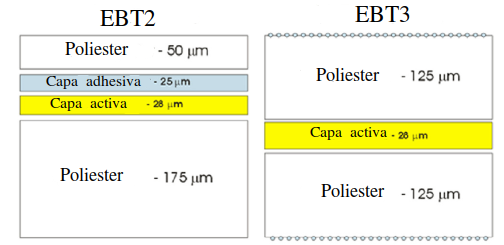
\includegraphics[width=0.45\textwidth]{images/estructuraEBT.png}
	\caption{Estructura de películas EBT\cite{Devic2016}}
\end{figure}
\end{frame}


\begin{frame}{Motivación}
	El uso de estas presenta varias ventajas
	\begin{itemize}
		\item Alta sensibilidad a la dosis(0.1 Gy-10Gy)
		\item Sin dependencia energética(50keV-10 MeV)
		\item Bajo costo y amplia variedad
		\item Practicas de usar
	\end{itemize}
\end{frame}

\begin{frame}{Objetivos}
	\begin{outline}
		\1 Entender y aplicar el funcionamiento de películas radiocrómicas en verificación dosimétrica
		\2 Realizar calibraciones de dosis
		\2 Obtener mapas de dosis de un tratamiento a partir de una película
		\2 Realizar la comparación con el plan esperado
		\1 Desarrollar un software que permita su uso bajo diferentes modalidades para su uso en el CCC
	\end{outline}
\end{frame}


\subsection{Tratamiento de películas radiocrómicas}
\begin{frame}{Modo de uso de películas radiocrómicas}
Para usar la películas hay que tener en cuenta ciertos factores ambientales que afectan las medidas
	\begin{outline}
		\1 Temperatura
		\1 Humedad
		\1 Orientación y posición de escaneo
		\1 Tiempo post-irradiación
	\end{outline}
Mantenerlos controlados basta para una medida precisa
\end{frame}

\begin{frame}{Calibración}
	Irradiamos la película con diferentes dosis conocidas, obtenemos cierta coloración por cada dosis
	\begin{figure}
		\centering
		\begin{minipage}{0.45\textwidth}
			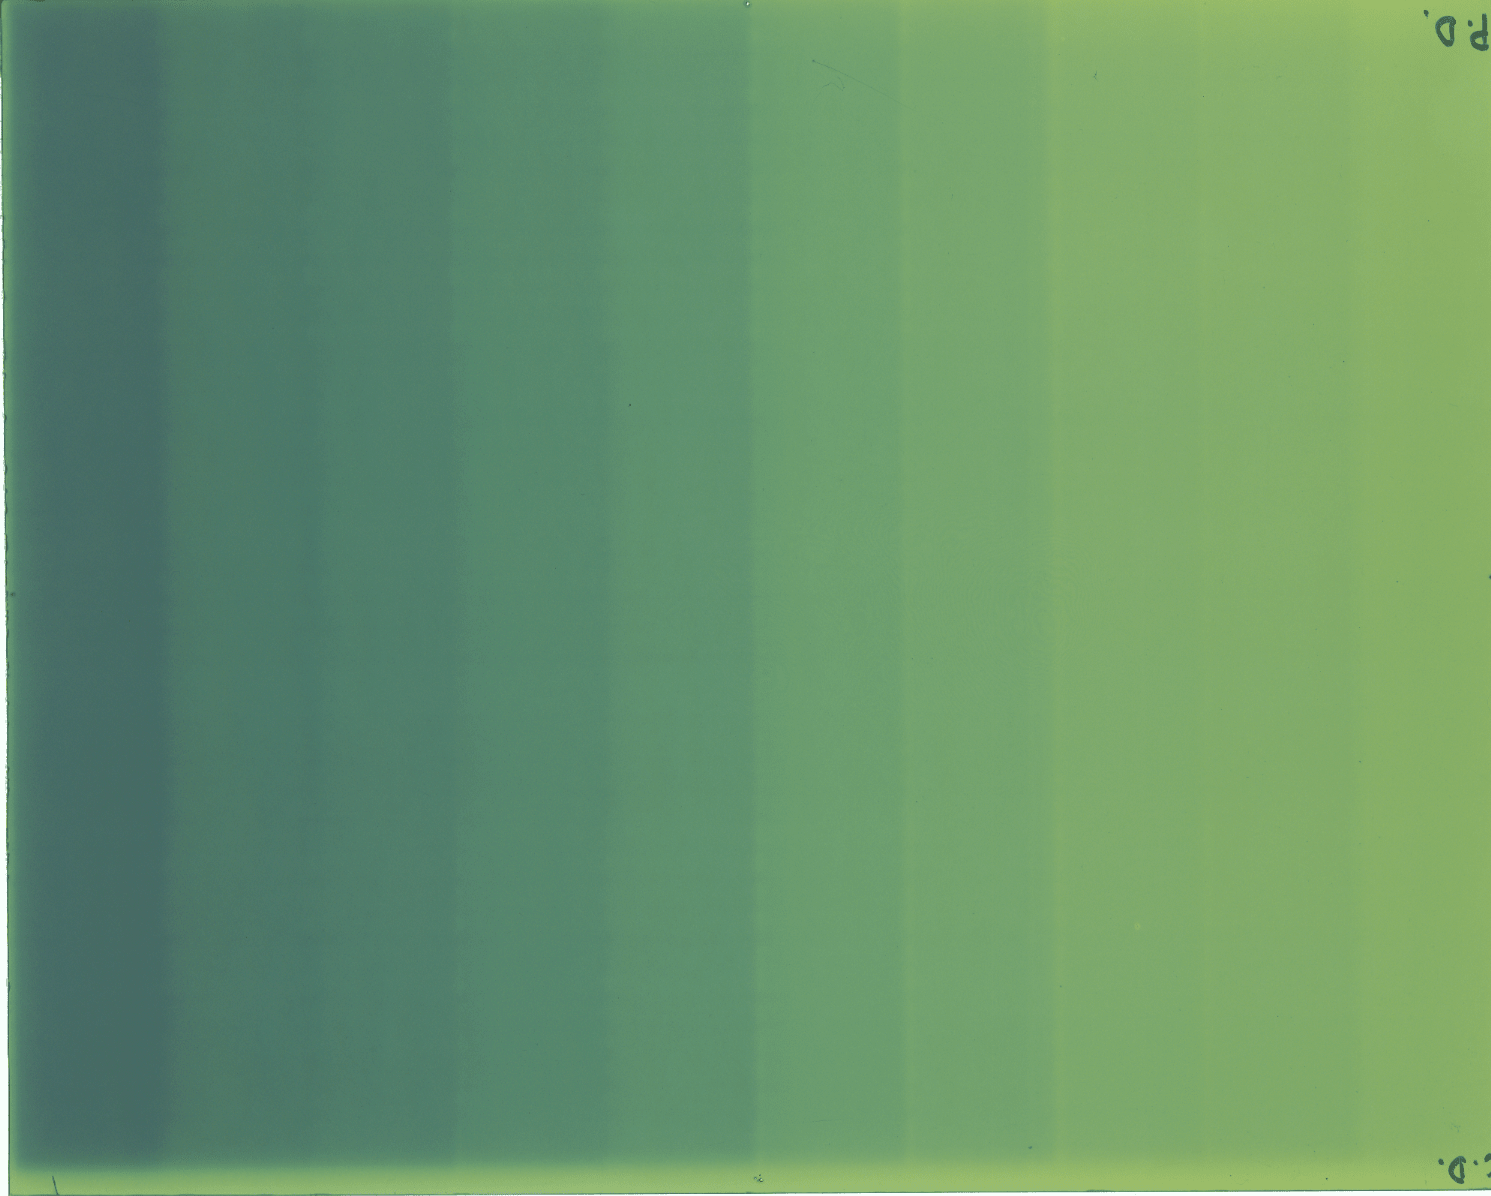
\includegraphics[width=\textwidth]{images/calibracionSimpleLandscape.png}
			\caption{Película de calibración}
		\end{minipage}\hfill
		\begin{minipage}{0.45\textwidth}
			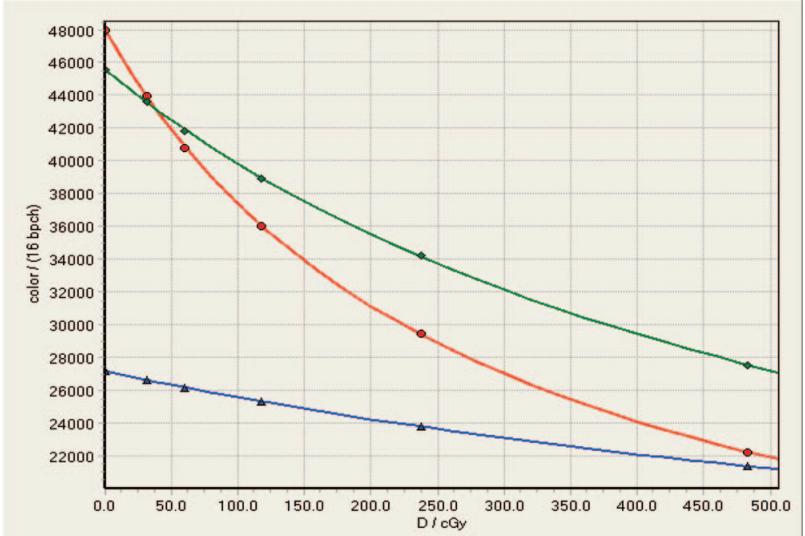
\includegraphics[width=\textwidth]{images/respses.png}
			\caption{Curva de respuesta\cite{Rink2008}}
		\end{minipage}
	\end{figure}
\end{frame}

\begin{frame}
	Se correlacionan los datos mediante un ajuste a algún tipo de curva.\\~\\
	Estos son los tipo de funciones más usadas
	\begin{itemize}
		\item Racionales 
		\item Polinomicas
		\item Inversas
		\item Lineal
	\end{itemize}
\end{frame}

\begin{frame}
	Con esta curva podemos relacionar dosis con colores en una película irradiada y generar mapas de dosis.\\~\\
	\begin{figure}
		\centering
		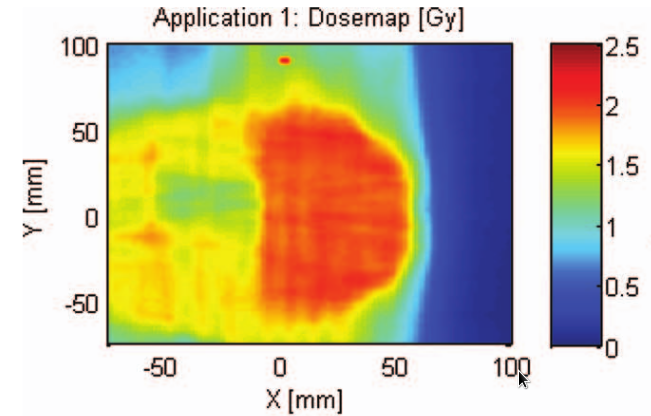
\includegraphics[width=0.7\linewidth]{images/dosemap.png}
	\end{figure}
\end{frame}


\begin{frame}{Métodos Corregidos}
Podemos sofisticar un poco con correcciones como 
\begin{itemize}
	\item Usar información de los tres canales para corregir inhomogeneidades
	\item Aplicar cambios en las curvas para incluir errores laterales en el escáner
	\item Filtrar las imágenes para corregir defectos
\end{itemize}
\end{frame}

\section{Avances}
\begin{frame}
	\vfill
	\centering
	\begin{beamercolorbox}[sep=8pt,center,shadow=true,rounded=true]{title}
		\usebeamerfont{title}\insertsectionhead\par%
	\end{beamercolorbox}
	\vfill
\end{frame}

\subsection{Toma de imágenes}

\begin{frame}{Montaje}
\begin{figure}[htp]% [H] is so declass\'e!
	\centering
	\begin{minipage}{0.45\textwidth}
		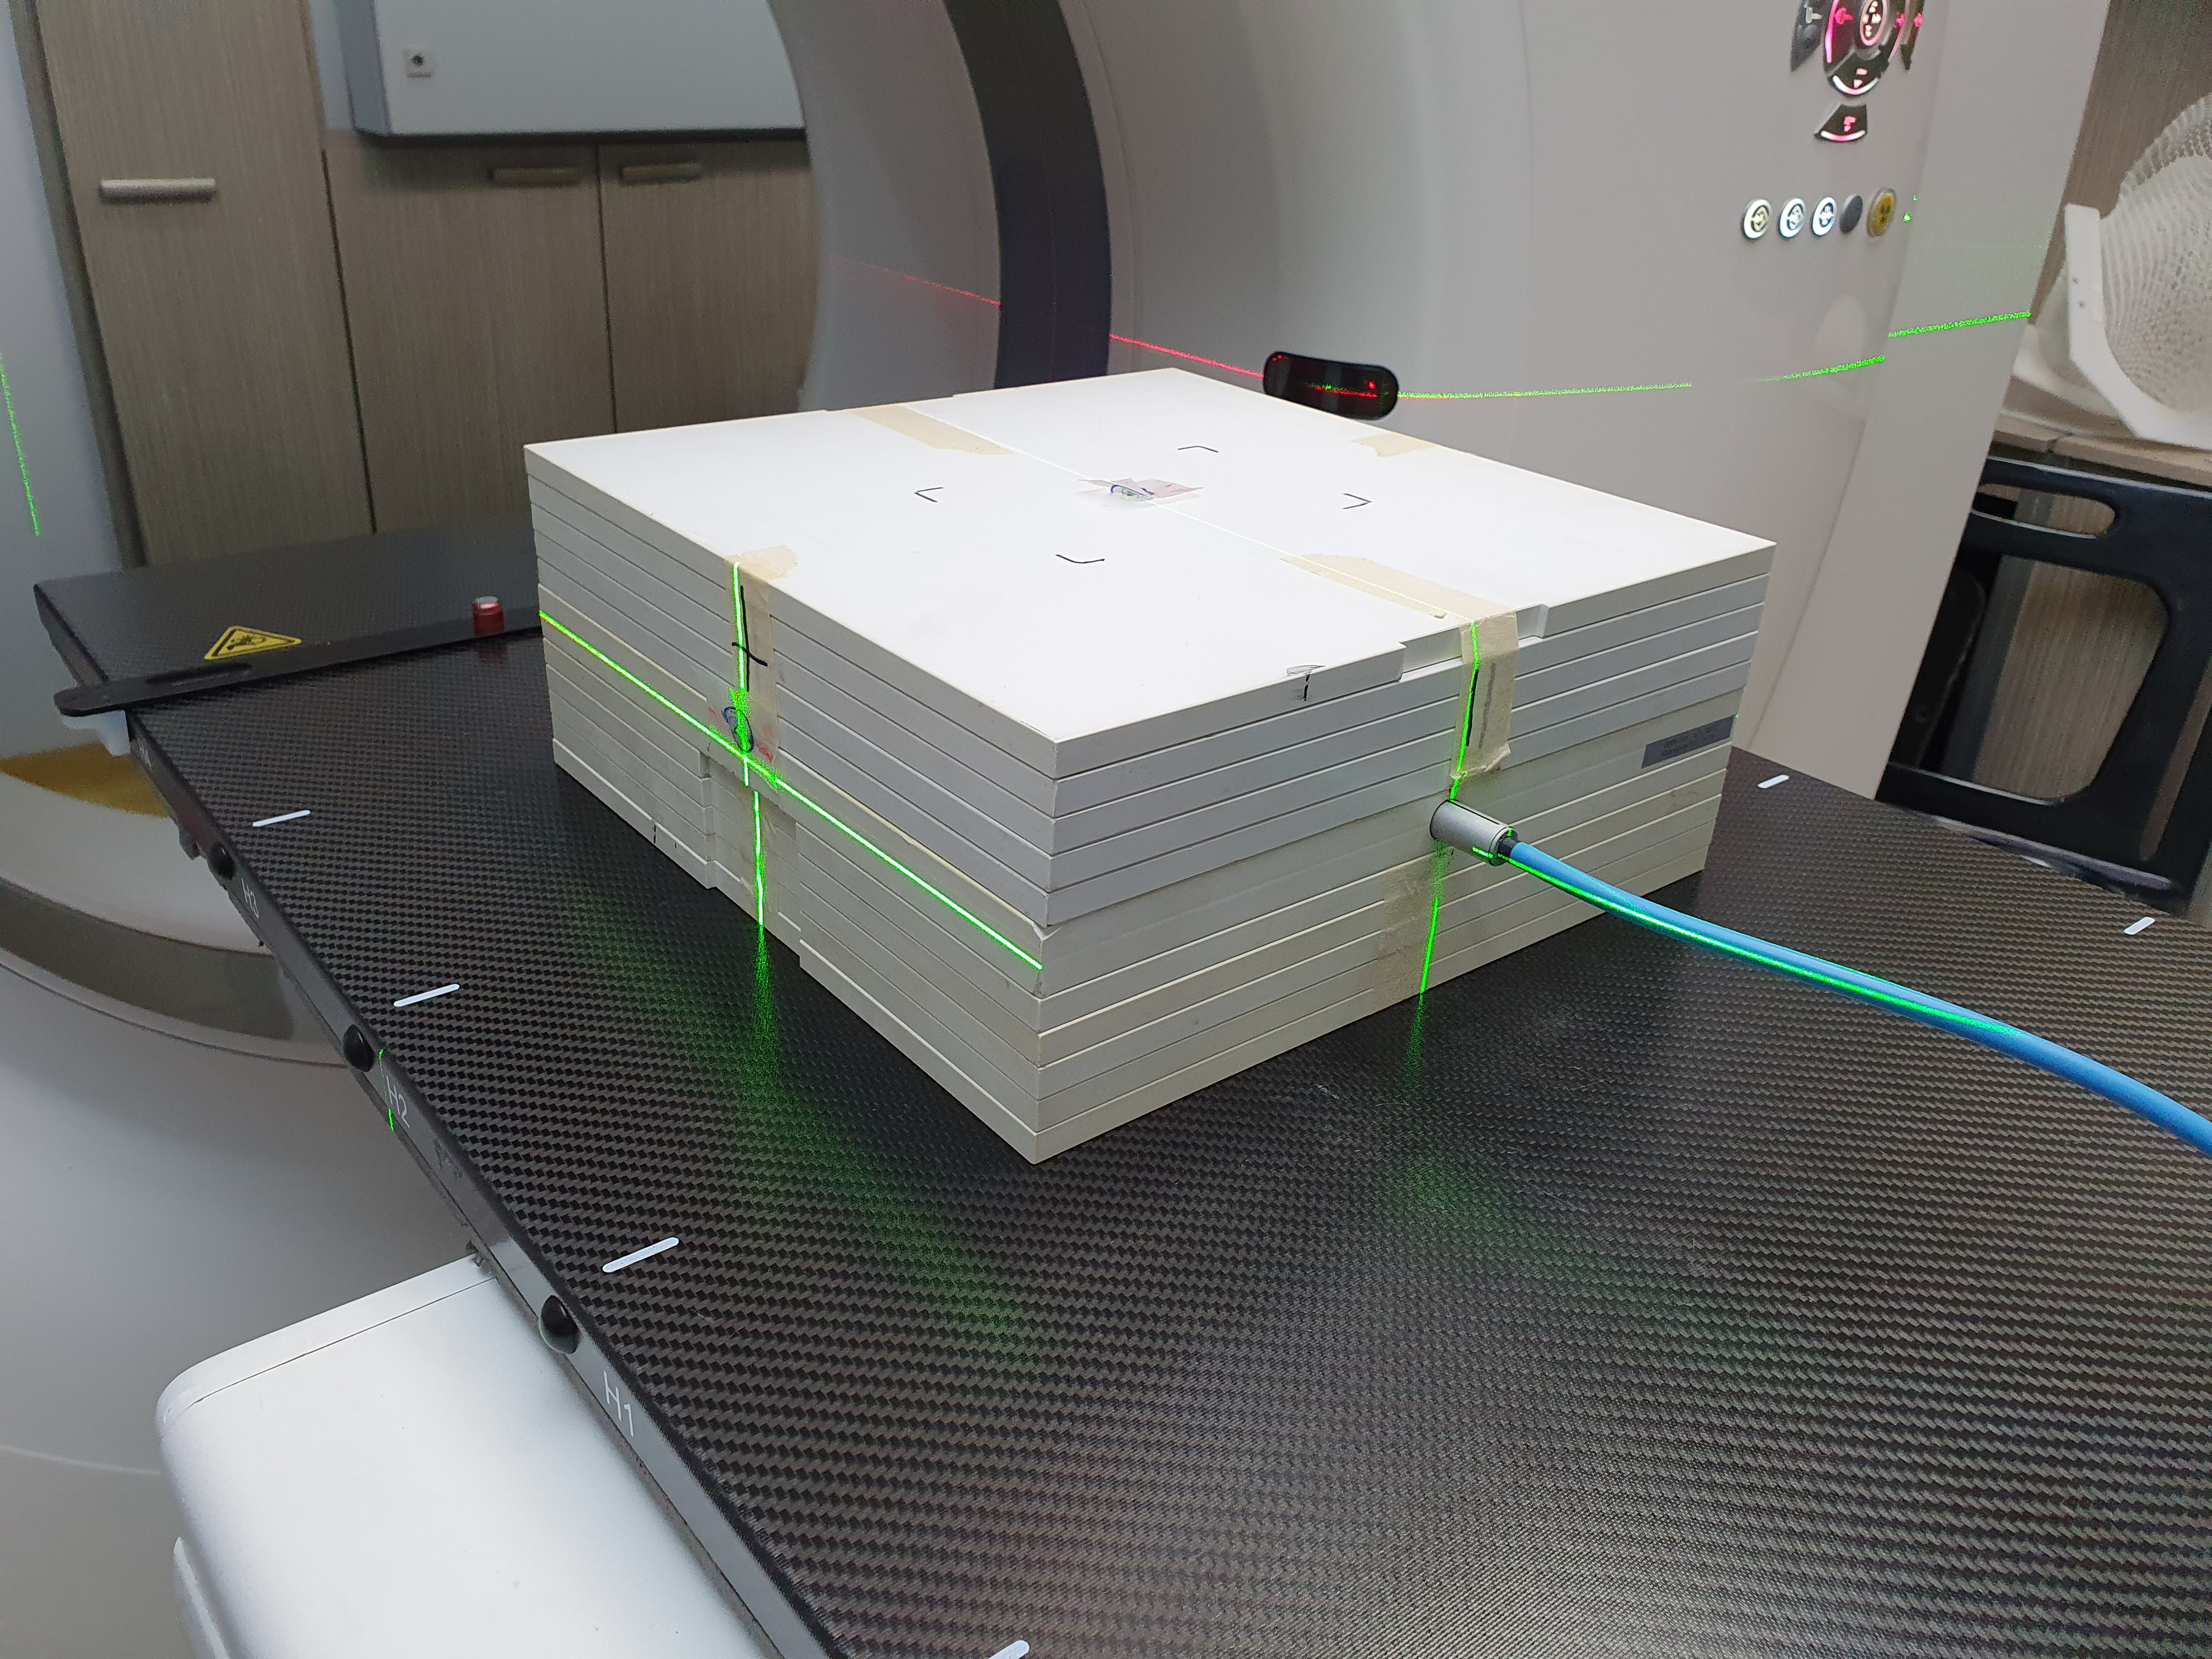
\includegraphics[width=\textwidth]{images/20200826_153715.jpg}
	\end{minipage}\hfill
	\begin{minipage}{0.45\textwidth}
		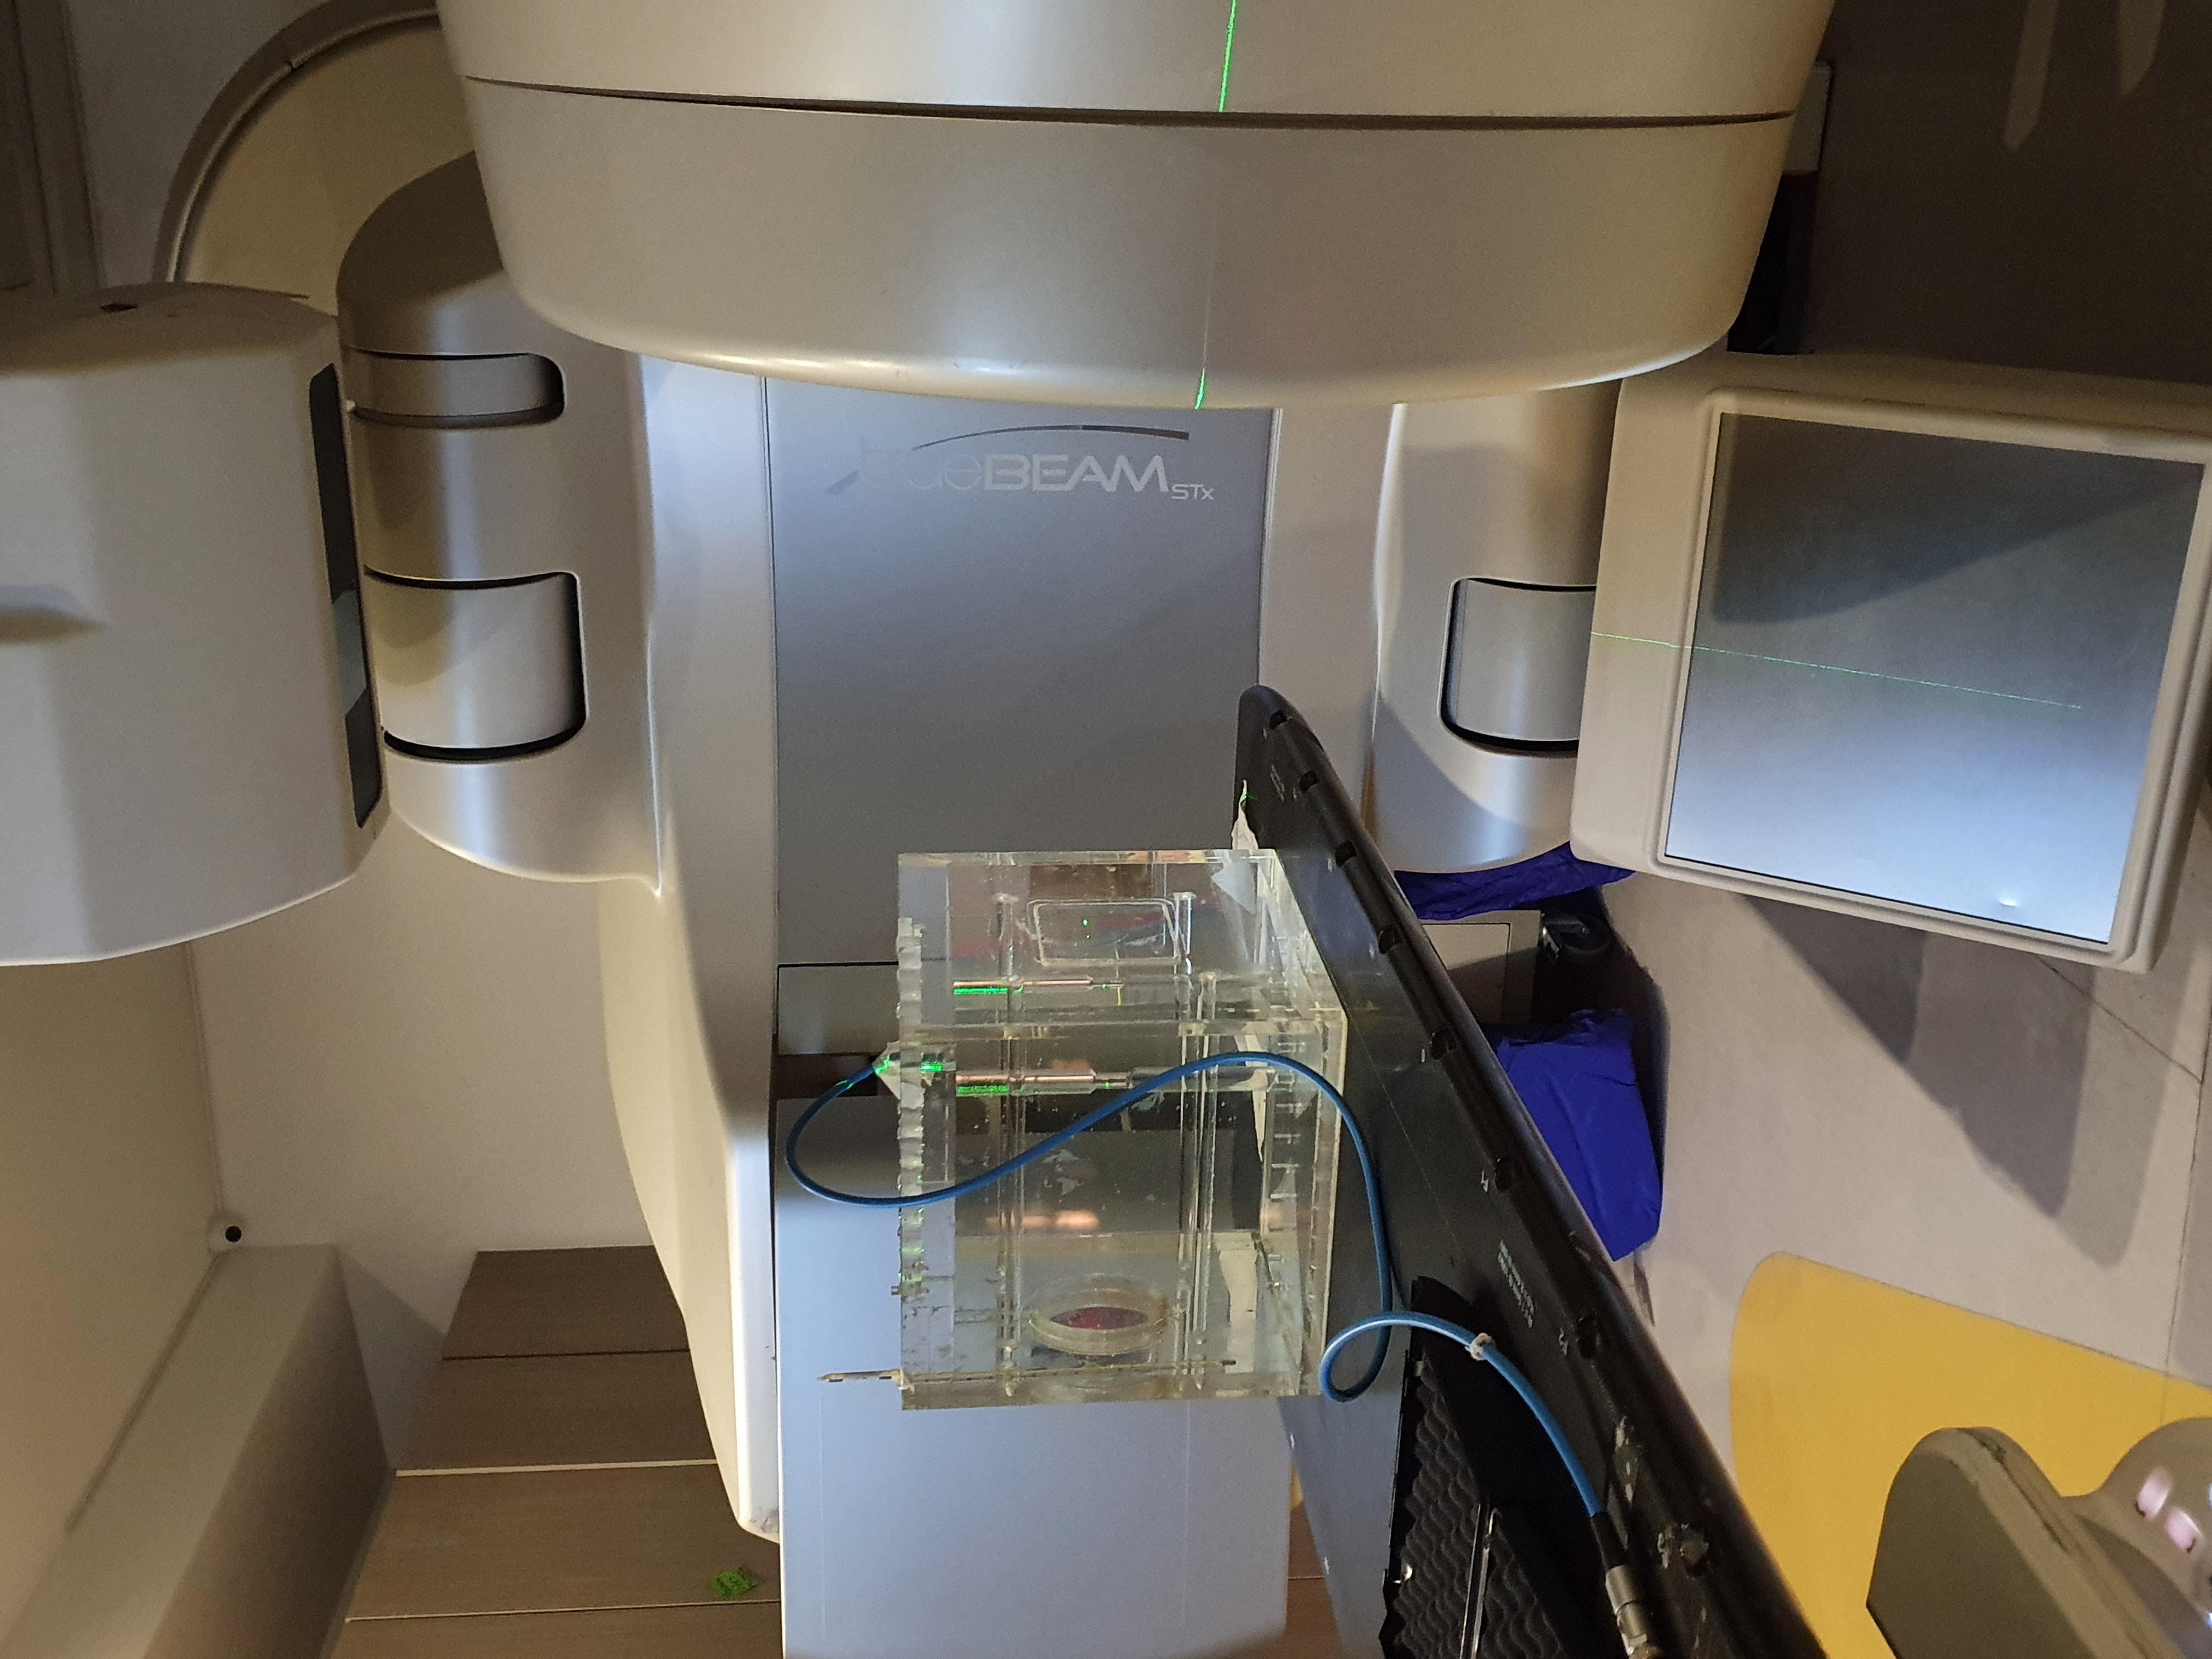
\includegraphics[width=\textwidth]{images/20200826_205548.jpg}
	\end{minipage}\par
	\vskip\floatsep% normal separation between figures
	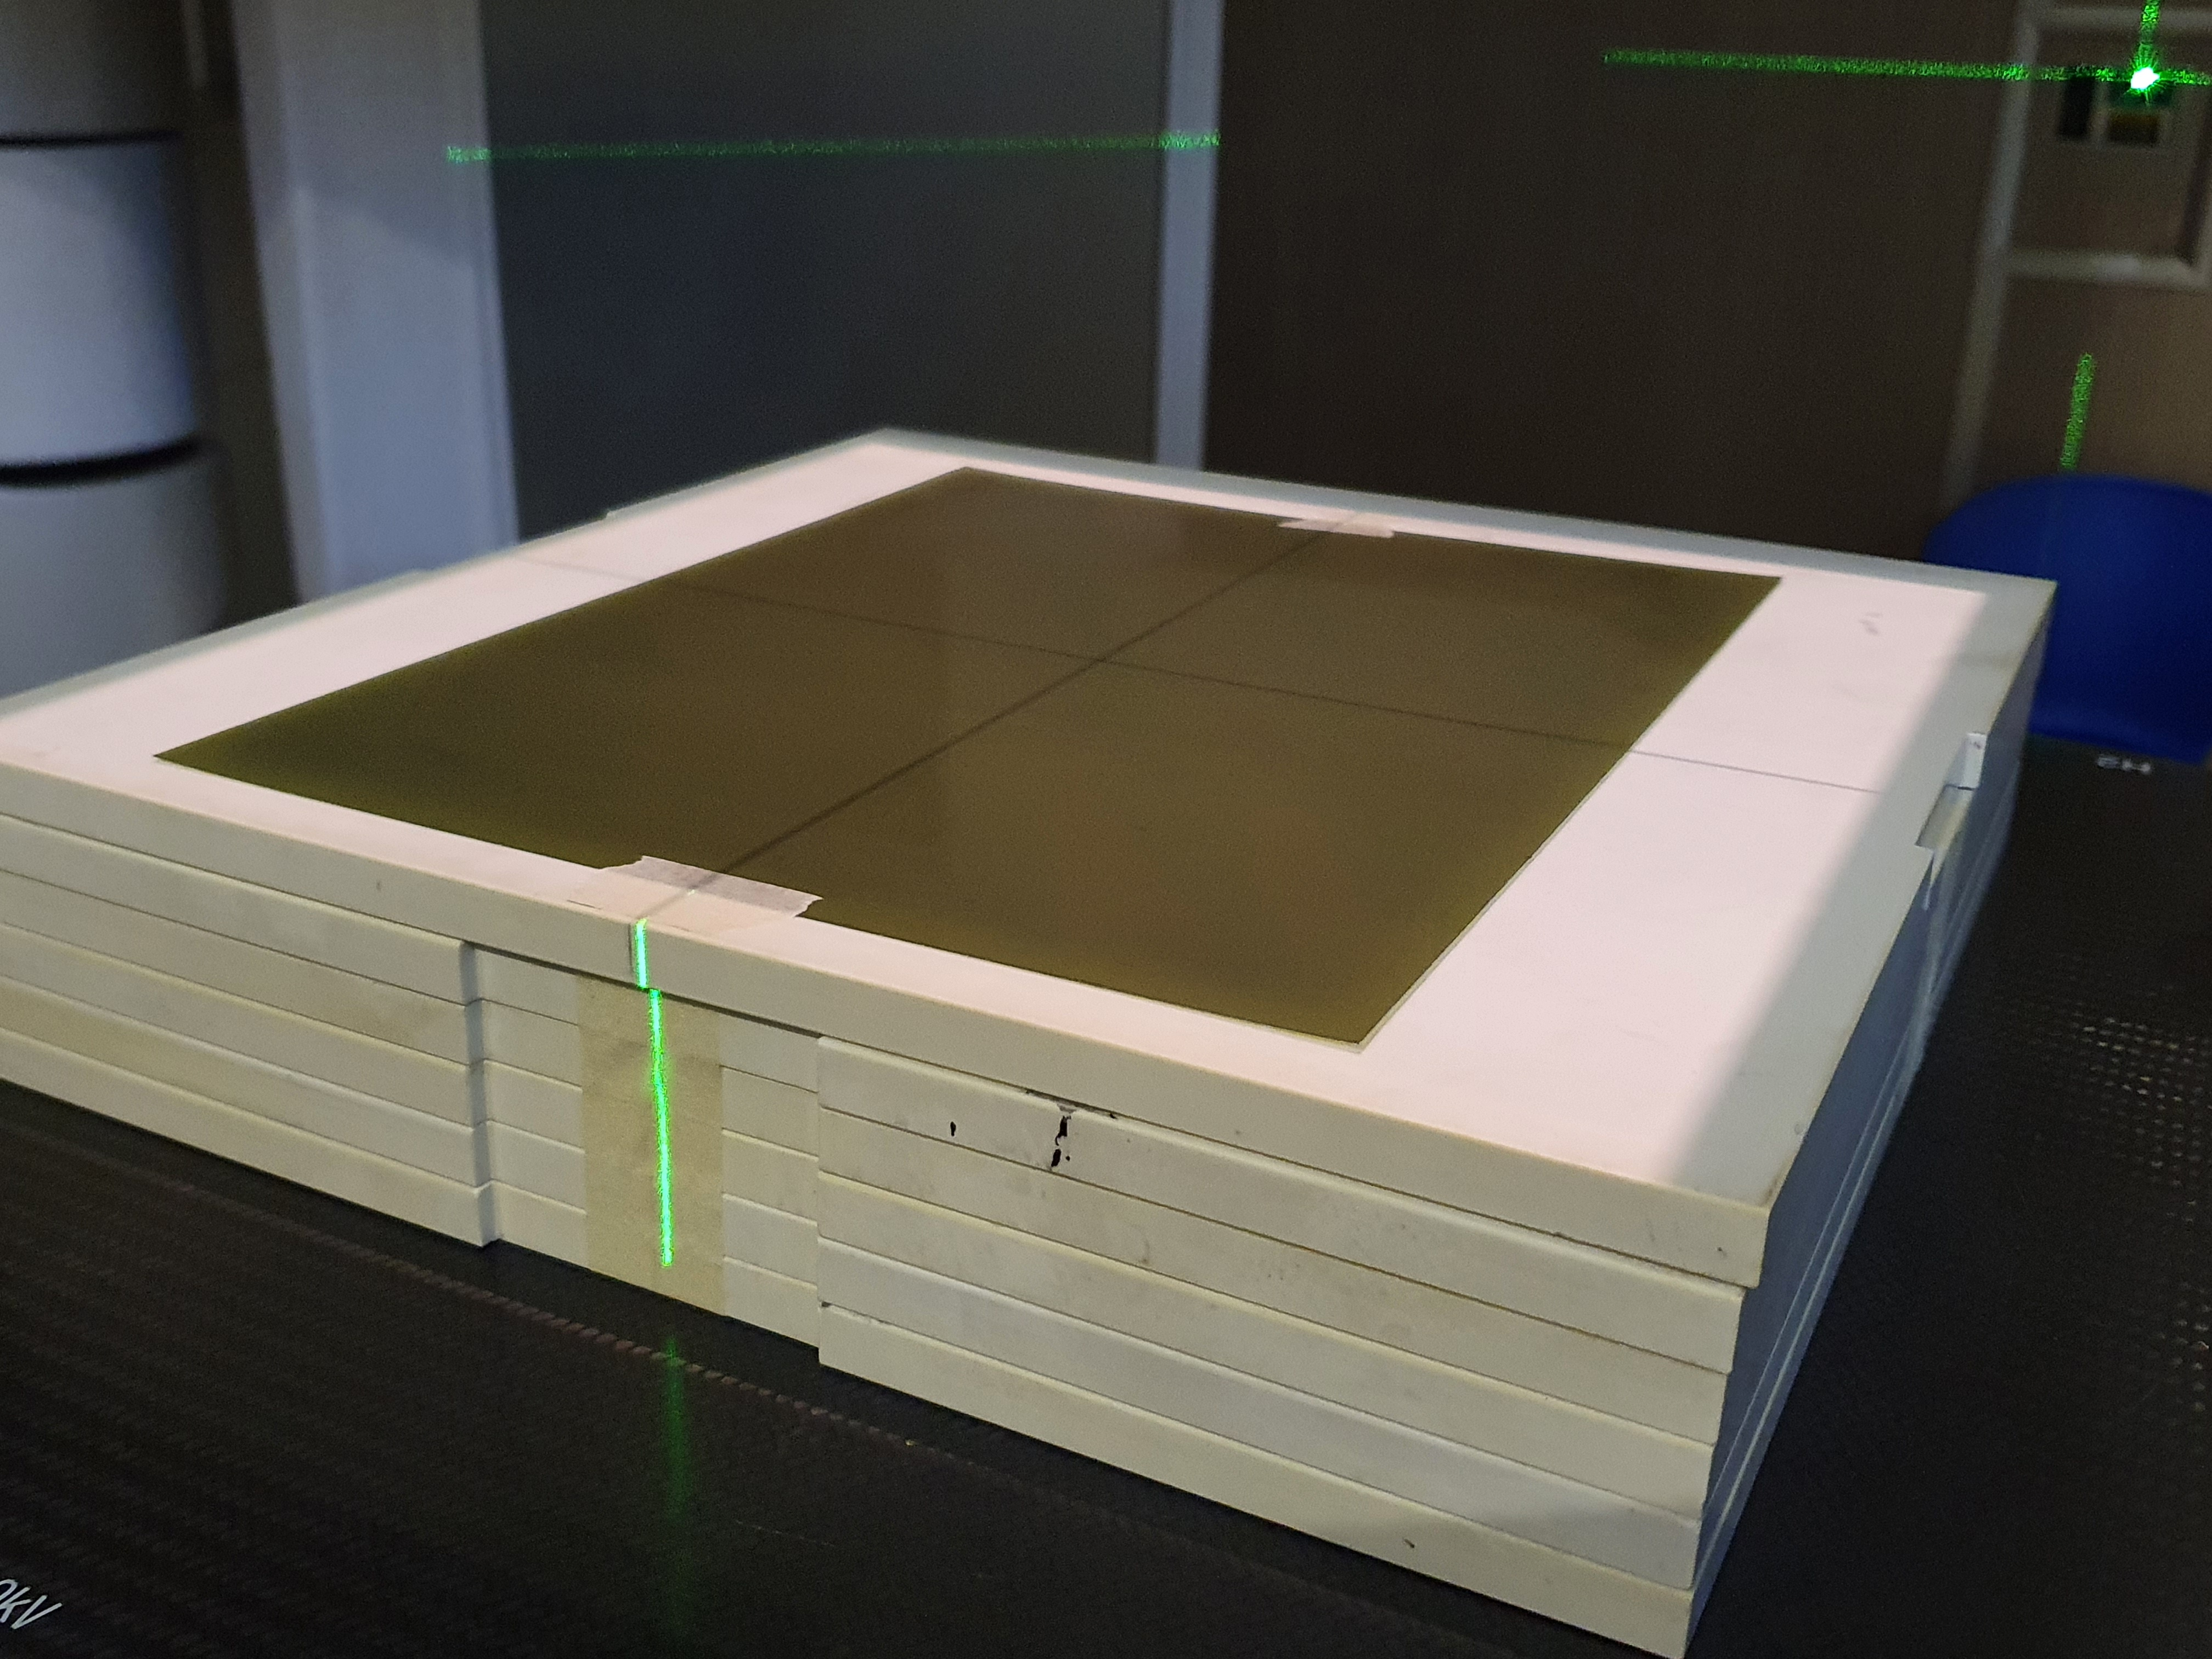
\includegraphics[width=0.45\textwidth]{images/20200826_215214.jpg}
\end{figure}
\end{frame}



\subsection{Desarrollo del software}

\begin{frame}{Montaje}
\begin{figure}[htp]% [H] is so declass\'e!
	\centering
	\begin{minipage}{0.45\textwidth}
		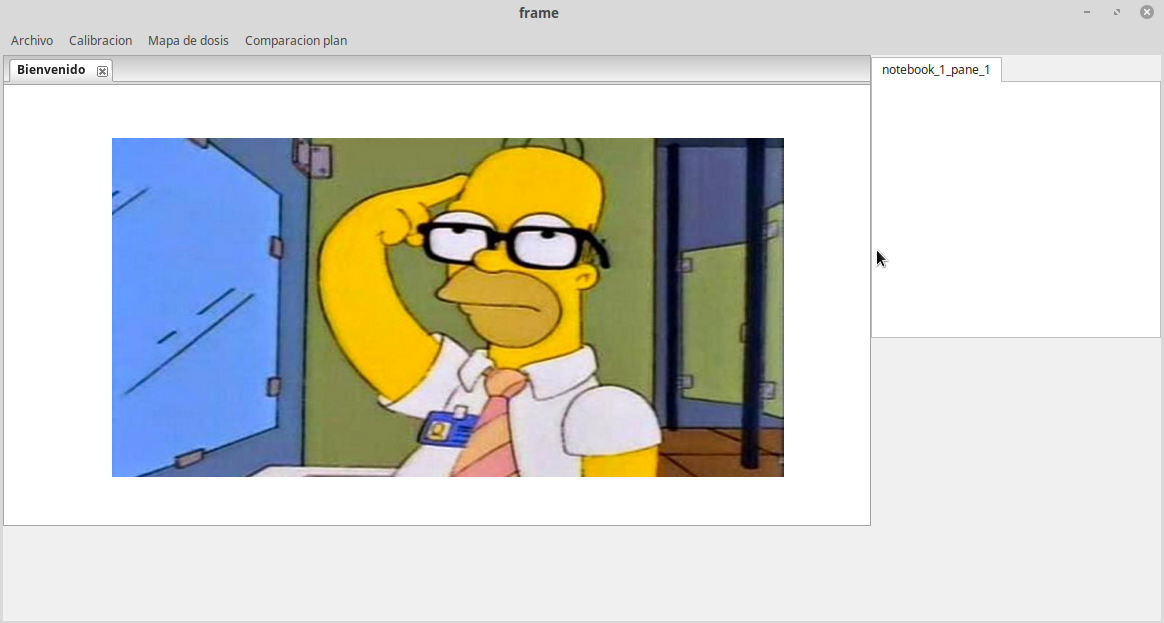
\includegraphics[width=\textwidth]{images/programa1.png}
	\end{minipage}\hfill
	\begin{minipage}{0.45\textwidth}
		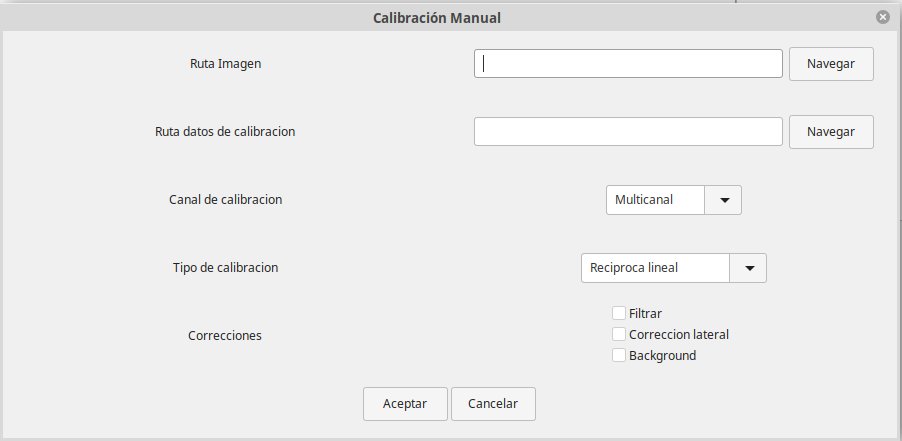
\includegraphics[width=\textwidth]{images/programa2.png}
	\end{minipage}\par
	\vskip\floatsep% normal separation between figures
	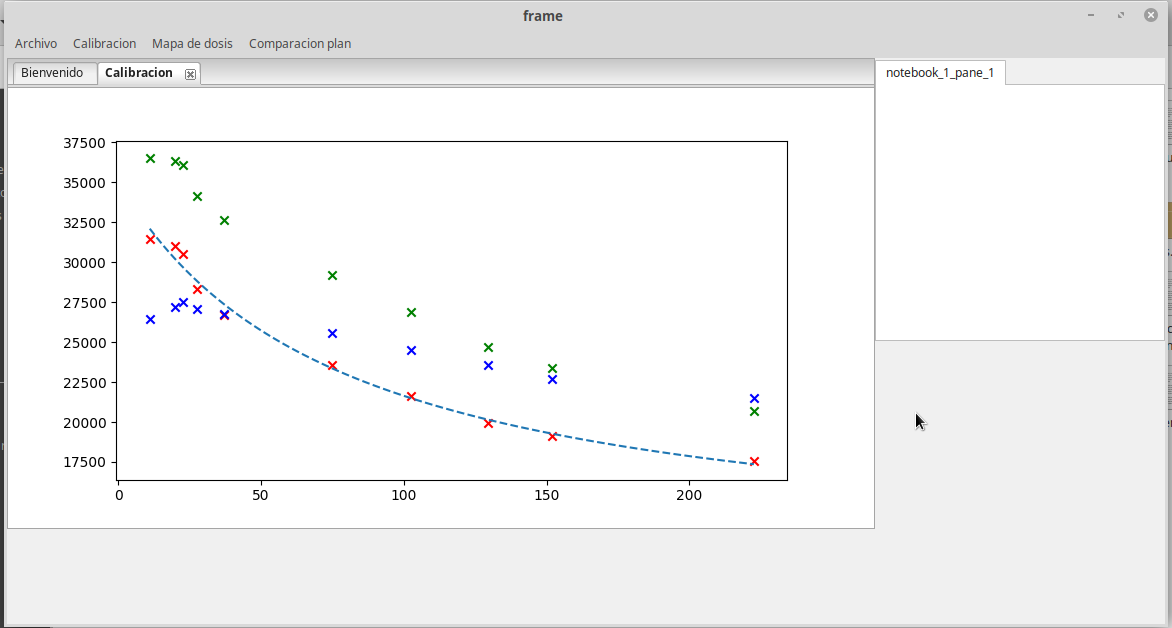
\includegraphics[width=0.45\textwidth]{images/programa3.png}
\end{figure}
\end{frame}

\begin{frame}
\begin{figure}
	\centering
	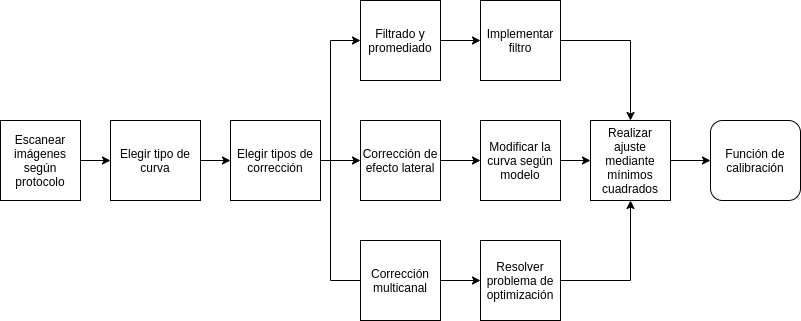
\includegraphics[width=\linewidth]{images/daigramaFlujo.png}
\end{figure}
\end{frame}






\section{Objetivos a cumplir}
\begin{frame}
\vfill
\centering
\begin{beamercolorbox}[sep=8pt,center,shadow=true,rounded=true]{title}
	\usebeamerfont{title}\insertsectionhead\par%
\end{beamercolorbox}
\vfill
\end{frame}

\begin{frame}
Porcentaje avance documento 40\% \\
Porcentaje cumplimiento objetivos 50\%\\~\\
Faltaría lo siguiente
\begin{itemize}
	\item Mejorar la usabilidad del programa (hasta el final)
	\item Generar mapas y curvas de isodosis (próximas 3 semanas)
	\item Entender e implementar el cálculo de $\gamma$ para la comparación cuantitativa con los planes de tratamiento(3 semanas)
\end{itemize}
\end{frame}



\section{Bibliografía}
\begin{frame}[allowframebreaks]
\frametitle{Referencias}
\nocite{*}
\bibliographystyle{ieeetr}
\bibliography{references}
\end{frame}



\end{document}